\section{Creating the Wonderless}
\label{dataset}

Figure\,\ref{fig:overview} summarizes the overall process of constructing Wonderless. 
The procedure consists of two main phases. 
We will thoroughly describe each of these phases in the following.

\begin{figure*}
	\centering
	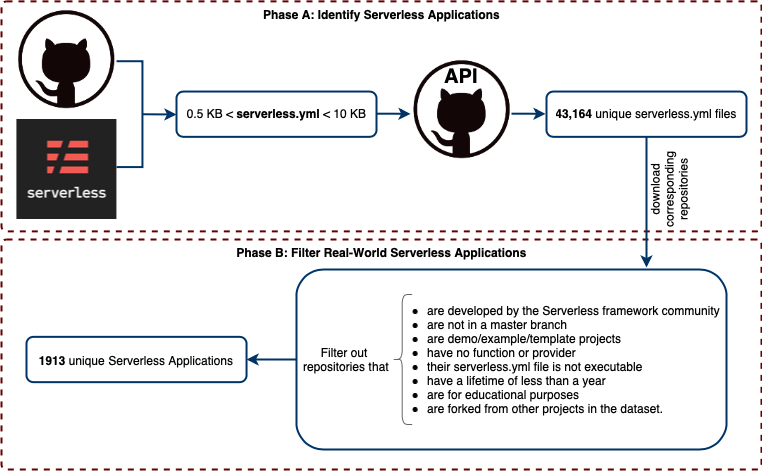
\includegraphics[scale=0.55]{figures/msr}
	\caption{Overview of creating Wonderless. TODO: let's discuss the picture}
	\label{fig:overview}
\end{figure*}

TODO: This section starts by describing how we did -not- create the dataset.
Should we move those parts to a discussion section?
I think we need to distinguish the process for achieving the research result and the 
research result itself.

\subsection{Identify Serverless applications} \label{phaseA}
The starting point for constructing the Wonderless is identifying Serverless 
applications. One way to achieve this end is to use services like 
GHTorrent\cite{gousios2012ghtorrent}, 
an offline mirror of the GitHub public event timeline, to search for repositories 
that contain specific keywords in their descriptions, topics, commits or other 
related attributes. The problem with this method is that containing a keyword 
does not necessarily guarantee that an application is Serverless. Besides, an 
application may be Serverless without containing a specific keyword in the 
attributes of its related repository.

The other way is to use GitHub API to search for a configuration file that is 
particularly for Serverless applications. The documentation of popular cloud 
providers reveals that the Serverless configuration file has the same default 
name as the configuration file for other cloud offerings. 
For example, one of the default Serverless configuration files in Amazon 
Web Services\,(AWS) is $index.js$. To this date\footnote{\today}, there 
are more than $135 \, M$ files with this name in GitHub, and they are not 
necessarily related to a Serverless application. To make matters worse, 
searching for this file will limit the dataset to only the applications supported 
by AWS. To include the Serverless applications provided by other vendors, 
one requires to search for the specific configuration files of those providers 
individually. This procedure can lead to a massive dataset with a large number 
of unrelated data points.

These challenges point to search for a configuration file that is first exclusively 
for Serverless applications, and second, it has the same default name across 
different cloud providers and Serverless platforms. 
$Serverless \; Framework$\footnote{\url{https://www.serverless.com}} 
with more than 36\,K GitHub stars and 15\,M downloads satisfies both these 
criteria. According to a review of Serverless frameworks\cite{kritikos2018review}, 
the $Serverless \; Framework$ with the highest number of supported providers 
and programming languages, and with the advance deployment, testing, 
monitoring, and security offerings is the most comprehensive existing framework. 
This framework uses a file with the YAML extension named $serverless$ 
by default as the configuration file, and it allows developers to deploy their 
applications to a cloud provider like AWS, Microsoft Azure, Google Cloud 
Platform, Apache OpenWhisk, Cloudflare Workers, or a Kubernetes-based 
solution like Kubeless.

Listing\,\ref{lst:example} represents an example of a $serverless.yml$ file. 
Depending on the chosen provider, this file can have many different properties.
The example shows the configuration properties for a telegram bot including 
name of the provider, runtime of the application, name of the function, 
and type of the event that triggers the function. The $serverless.yml$ file is 
not unique for each application, meaning that an application can have separate
$serverless.yml$ configuration files for different services.

\vspace{2mm}

\begin{lstlisting}[frame=single, caption=An example of a serverless.yml file., label={lst:example}, captionpos=b]
service: azure-telegram-bot 

provider:  
	name: azure
	runtime: nodejs12.x  
	
plugins:  
	- serverless-azure-functions 

functions:
	hello:    
		handler: (*@handler.hello@*)
		events:   
			- http: true        
			   x-azure-settings:          
			   		authLevel: anonymous
\end{lstlisting}

\vspace{2mm}

We used GitHub API to search for all the $serverless.yml$ files in GitHub. 
Since GitHub API has a limitation of $1000$ results per query, we structured 
the query into subqueries based on the size of a file. 
Due to this, we searched for all the $serverless.yml$ files that are larger 
than $0.5\,KB$ and smaller than $10\,KB$. The files with less than 
$0.5\,KB$ are mostly empty, and there are barely such files that are 
larger than $10\,KB$. As the result of our search on July 29, 2020, 
we collected the URL of $43,164$ unique files, corresponded to 
$30,489$ unique repositories. Using the URLs, we cloned 
the repositories to create the initial version of the dataset that 
resulted in $\sim 400 \, GB$ of data.

\subsection{Filter real-world Serverless applications} \label{phaseB}
The initial dataset included a large number of ineffectual data points 
such as inactive and toy projects. To end up with real-world Serverless 
applications, we applied several rounds of filters to the dataset.

As the first step to elude bias in the dataset, we checked the developers 
of applications and removed a repository if the repository was developed 
by the $Serverless \; Framework$ community. 

Next, we looked into the structure of the repositories. 
For avoiding unstable applications, we removed a repository if it was not 
on the main branch. In addition, to remove the applications that served 
presentation purposes, we removed a repository if the configuration file 
of the repository was placed in a directory that contained one of the 
\emph{example}, \emph{demo}, \emph{template}, or \emph{test} 
keywords in its label.

Then, we used a python script to make an initial analysis of the 
configuration files. We looked for the results of three metrics in this 
analysis: \rom{1}) if the configuration file is executable, \rom{2}) if 
the configuration file has the name of the provider property and 
\rom{3}) if the configuration file contains the information for any 
function. We removed a repository if its configuration file was not 
executable, had no particular provider, or had no specified function.

By the end of this step, the dataset had $371 \, GB$ of data consisting 
of $27,812$ unique repositories. To eliminate inactive projects, we 
removed a repository if the lifetime of the repository was less than 
a year. We used $git \; log$ to view the commit history of repositories. 
For each repository, we defined the lifetime of the project as the difference 
between the date of the last commit and the date of the first commit. 
Figure\,\ref{fig:lifetime} demonstrates the distribution of lifetime of the 
projects in the dataset. As it is shown, more than $70\%$ of the projects 
in the dataset were active for less than a month. Overall, more than $90\%$ 
of the project did not have a new commit a year after the initial commit. 
This step dramatically reduced the size of the dataset.

\begin{figure}
	\centering
	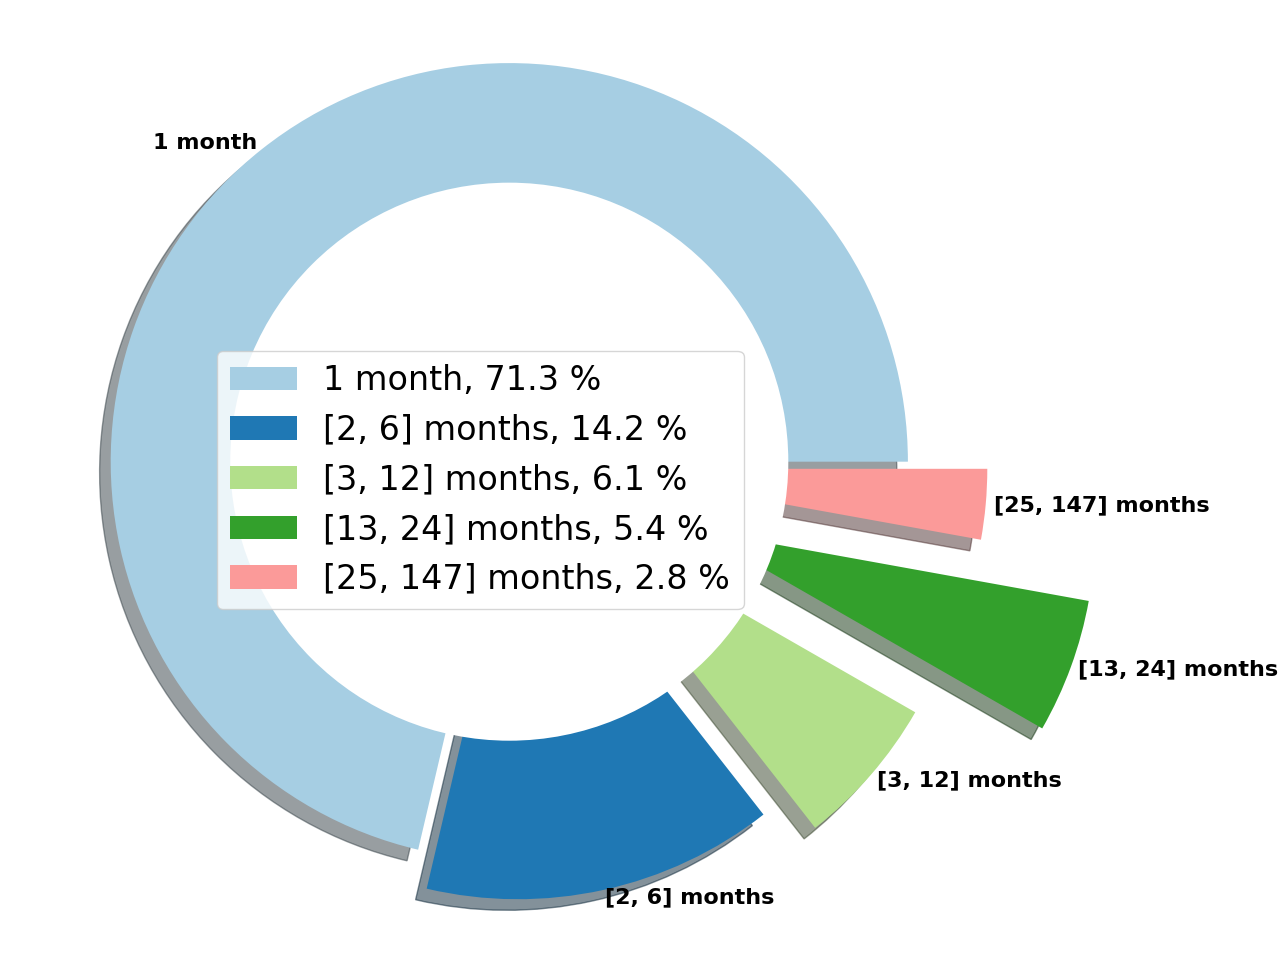
\includegraphics[scale=0.25]{figures/lifetime}
	\caption{Distribution of lifetime of the Serverless applications.}
	\label{fig:lifetime}
\end{figure}

To eliminate the projects developed for educational reasons, 
we applied a keyword search to the labels, topics, and 
descriptions of repositories. We extracted the description 
and topics of each repository using $mercy-preview$ media 
type of GitHub API previews. We removed a repository 
if the repository contained one of the following keywords: 
\emph{example, demo, tutorial, playground, learn, teach, exercise, 
	course, practice, template, sample, workshop, lecture, study}.

Finally, to avoid duplications, we removed a repository if it was forked 
or copied from other repositories in the dataset. To do this, we automatically 
searched for the projects with the same name and different developers. 
Then we manually checked if those repositories were actually the same or 
they accidentally had the same name. If two repositories were the same, 
we removed the one with fewer commits or fewer contributors.

We describe the structure of Wonderless in the next section. 
In section\,\ref{limitations}, we discuss the limitations of our dataset, 
and we introduce the potential use cases of Wonderless in section\,\ref{usecase}.